% !TeX spellcheck = en_US
\chapter{Literature Review}
\label{chp:back}
% Why use CPP for the SAR problem
% Give some kind of intro to CPP and the different approaches - Surveys
% zhang paper
% What is motion planning - Lavalle
% online vs offline etc.
As mentioned in section \ref{sec:intro_bg}, \acl{cpp} is a subset of the general motion planning problem. This chapter will therefore begin with a brief overview of motion planning before discussing \acs{cpp} as a whole. Literature pertaining to \acs{cpp} is then discussed in several sections. Firstly, it is addressed in the context of the single robot \acs{cpp} problem. Several techniques used to achieve coverage using only one robot are summarized. Following this are three sections dedicated to \acf{mcpp} problem. The first two cover distributed and non-distributed offline \acs{mcpp} respectively. This is followed by a section presenting some online \acs{mcpp} implementations. Many of the implementations were done with some application in mind, but the last section covers \acsp{uav} and how they have been applied to \acs{sar} operations in particular.
% TODO: Check Acronyms

\section{Motion Planning}
Perhaps one of the most noteworthy items of literature presented on motion planning is \cite{Lavalle2006}. In this book, a differentiation is made between motion planning and trajectory planning. Motion planning, by their definition, refers to a series of translations and/or rotations required to get an agent from one point to another within some environment. Trajectory planning would then take this plan and find a strategy to execute it within the dynamic constraints of the agent. \emph{Agent} is a term from the field of artificial intelligence and is interchangeable with \emph{robot} or \emph{decision maker}.

% Motion planning
The book refers to planning algorithms as a strategy that is used by one or more decision makers to move from some starting state to some goal state within some context. State is a very general term and can refer to a number of different implementations. An example would be a robotic arm, the decision maker, that needs to move from some starting orientation, or state, to a goal orientation. Another common scenario involves simple start-goal path planning. An example would be a car that needs to travel from one point in a city to another. Here, the car is the decision maker (or agent) and a strategy needs to be found to move the car along some valid path to get from one point to another within the context of the city. Generally, it is favorable to try and find the shortest viable path in this kind of scenario.

% Environment - Discrete vs Continuous
In most applications, the environment wherein the agent exists is important to determine a valid strategy to reach the goal state. For the robotic arm scenario, it is important that the location of any obstructions within reach of the arm are known so they can be avoided. This kind of collision avoidance is important for the car as well. It must know where valid paths lie within the city to avoid collisions and stay along the road. The environment is generally either represented as discrete or continuous, depending on the planning algorithm.

% Online vs Offline
Information about the environment can be available a priori, in which case it is referred to as offline planning. This means that all information about the environment and its dynamics are known before execution of the planning algorithm. For the car, this would mean that before executing the path, all the obstacles in the environment are known. Dynamic obstacles e.g. other moving cars, would have their future positions and velocities mapped out beforehand as well. The planner can thus take these into account during the planning phase, prior to execution of the plan. Online planners also exist, where the environment is an unknown, or is only partially known a priori. This usually means the agent must have onboard sensors to map out its environment as it moves through it. This is often applicable in scenarios where actions by the agent change the environment or when there is a moving target with an unknown trajectory.

% Types of Multiple Robot Tasks
Motion planning can be extended to multiple agents in a single environment. Optimizing paths in these scenarios can be quite challenging, because agents must now not only avoid collisions within the environment, but also with one-another, while trying to achieve a certain goal. In the context of path planning with \acsp{uav}, the nature of the goal makes the problem fall into different categories, according to the authors of \cite{Zhang2020}. 

In a start-goal problem, if the goal location is the same for all \acsp{uav}, it is referred to as a rendezvous task. If they all have different goal locations, it is an allocation task. And lastly, if the goal is not to move from a starting position to a goal, but instead to cover every point in an environment, it is called a coverage task. The initial positions of the \acsp{uav} can also be  classified into aggregated or dispersed. Respectively, these refer to all the UAVs starting at the same position or starting at different locations within the environment.
% TODO: put in more references

% Decentralized vs Centralized - organizaional framework used to make decisions. Lauren used it for collision avoidance. Depends on the task what information is collected. Centralized means one central UAV collects information from ALL UAVs and makes decisions for ALL of them based on this - more processor intensive. Decoupled or decentralized means each UAV has autonomy and makes its own decisions based on its neighbours - this is probably what you would use.

% Complete
Once an algorithm is designed to apply to a specific scenario, its effectiveness can be measured ina  number of ways. Firstly, completeness refers to an algorithm that will always find the solution for a scenario, if one is possible\cite{Lavalle2006}. Another important measure is efficiency, which can be improved by making an algorithm run faster. Lastly is robustness, which indicates how resistant an algorithm is to failure \cite{Hazon2005}. 

%%%%%%%%%%%%%%%%%%%%%%%%%%%%%%%%%%%%%%%%%%%%%%%%%%%%%%%%%%%%%%%%%%%%%%%
\section{Coverage Path Planning}
% Description of offline vs online and mention that the next sections are offline, offline and online
% Maybe present more detail on algorithm complexities. Can they handle large grids and how many robots etc.
Coverage path planning algorithms can usually be classified into online or offline. These classifications refer to the amount of information available about the environment that needs to be covered \cite{CPP-Survey-2019}. Online planning is a dynamic approach wherein information about the environment is gathered during deployment and is not known a priori. Offline planning generally means that the environment is mapped out in full a priori. Robot trajectories for area coverage are planned prior to execution. Hybrid applications exist, wherein some information is known beforehand, but changes in the environment, for example moving obstacles or targets, can be collected and accounted for dynamically during execution \cite{Kamrani2014}.

%In multi-robot scenarios, the most notable challenge that comes into play is collision avoidance. Robots need to cooperate for area coverage without colliding with each other and any obstacles in the environment.
%Online planning has the advantage of detecting when collisions would happen in real time and then planning to avoid them. However, when using an offline approach, one must predict collisions pre-emptively. If there is then a prediction error, the result could be unfavourable. Therefore, an alternative, more optimum solution is suggested for offline problems. This is the divide areas approach, where an area gets divided between robots so that their paths would never cross.

%%%%%%%%%%%%%%%%%%%%%%%%%%%%%%%%%%%%%%%%%%%%%%%%%%%%%%%%%%%%%%%%%%%%%%%
\section{Single Robot Coverage Path Planning}
\label{sec:lit SR CPP}
This section is divided into subsections based on....
% Choset Taxonomy? Note that there are other categorisations, online vs offline, discret vs continuous, complete, resolution complete, probabilistically complete... 
% Mention simple maneouvres
\subsection{Exact Methods}
\label{sec:lit SR CPP - Exact}
An early form of coverage path planning can be found in \cite{Choset2001}. This is known as exact cellular decomposition. This was originally used for single robot applications where an area is divided into polygons, called cells, which are then searched sequentially by a single robot using simple back and forth motions. This is known as an exact solution because the area is still treated as continuous space and is not discretised as with approximate methods. Therefore, it is possible to get complete coverage of an area. The boustrophedon and trapezoidal decomposition are well known exact cellular techniques.\\
\subsection{A* Path Coverage Path Planning}
\subsection{Spanning Tree Coverage Path Planning}
\label{sec:lit SR CPP - STC}

\subsection{Wavefront Planning}
\subsection{Artificial Intelligence Based Planning}

%%%%%%%%%%%%%%%%%%%%%%%%%%%%%%%%%%%%%%%%%%%%%%%%%%%%%%%%%%%%%%%%%%%%%%%
\section{Distributed Offline MCPP}
\label{sec:lit Ditributed MCPP}
A well established offline coverage path planning approach involves the divide areas technique. This partitions an area into regions for individual robots to cover. Each robot should then be able to cover its area using one of the individual area coverage techniques mentioned in section \ref{sec:lit SR CPP}.
%This removes the need for collision avoidance, seen as the robot paths should never overlap. It is important in this kind of application that an individual robot starts its search path within the area that is allocated to it. \\
%Distributed vs Free - give the definitions of these for the purpose ofthis paper

\subsection{Hexagonal Segmentation}
 A notable distributed approach uses regular hexagons to segment the area of interest \cite{Azpurua2018}. This implementation is reminiscent of the exact methods often used for single robot coverage path planning mentioned in section \ref{sec:lit SR CPP - Exact}. Exact methods generally divide an area into arbitrarily sized polygons called cells. The robot moves between these cells and covers them using simple motions. In the multi-robot scenario, the area is still divided into cells, but they need to be distributed between the robots evenly for searching. The idea is to assign equal sized areas to each robot so that their path lengths are similar and they can complete their paths at roughly the same time.

Hexagonal cells make it easier to assign cells to robots, seen as they are all of the same size. Hexagons are clustered using the K-means algorithm to ensure a similar number of cells are assigned to each robot. The seeds are synonymous with the robots, therefore once the seed locations are finalised for even cell distribution, the robot initial positions are established. The robot initial positions cannot be at any random location, which is a drawback of this implementation. 

The hexagons that are assigned to a given robot are contiguous and form a subregion that is then covered using simple maneuvers. Generally, back and forth motions are quite popular. Static obstacles are considered in this implementation, but the smallest obstacle resolution is the size of an entire hexagon, which is another drawback to this implementation. Figure \ref{fig:Hex} illustrates the back and forth maneuvers used to cover the hexagonal partitions. Black hexagons represent no-fly zones and/or static obstacles. The dark red, green and blue regions represent the regions as they are assigned to the respective robots for coverage.

\begin{figure}[h!]
	\centering
	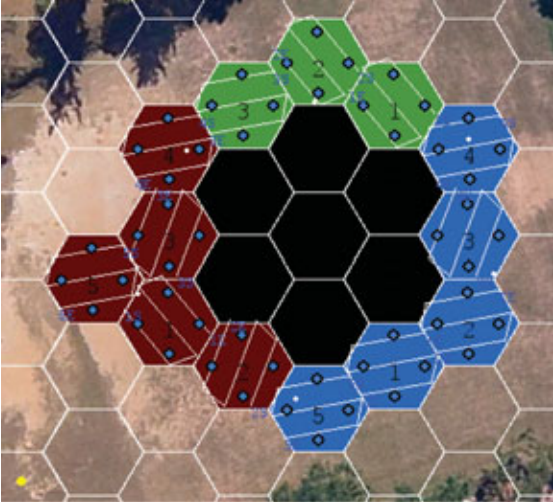
\includegraphics[scale=0.4]{figs/Hexagonal_Partitioning_Graphic}
	\caption{Simulation showing coverage of hexagonal partitions with back and forth motions with three robots. \cite{Azpurua2018}}
	\label{fig:Hex}
\end{figure}

\subsection{Voronoi Partitioning}
% Polygons
The individual path, to cover an area assigned to a robot, does not have to use simple motions. Often times, emphasis is placed on the area division algorithm and the single robot coverage paths are somewhat arbitrary. Those paths can be planned using any number of the single robot algorithms such as those mentioned in section \ref{sec:lit SR CPP}. In the mathematics field, there is work surrounding area division where they devise a method to divide a polygon into equal area polygons of a certain amount \cite{Nandakumar2012}. An old, but relevant, method that also stems from the field of mathematics, is the Voronoi partition. This assigns regions within an area to seeds based on distance. The idea is that a region assigned to a seed represents all the points where the distance to that seed is shorter than to any other seed.

% Voronoi
If the Voronoi partition is applied to the MCPP problem, the seeds once again become synonymous with robots. This partition works for any number of robots at any starting positions, but unless they are evenly spaced, the areas will all have varying sizes. Distances in these scenarios are usually Euclidean and the boundaries between areas represent the position where the distances from two seeds are equal. The authors of \cite{Nair2020} implement MCPP using Voronoi partitions in discrete space with static obstacles. They used square discretisation of the area and compared several different methods. They investigated geodesic-Manhattan-, Manhattan-, geodesic- and Euclidean-distance-based Voronoi partitions. 
% TODO: EDITING - Euclidean and Manhattan should always be with a capital letter 

Due to obstacles in the area, the Euclidean-based technique resulted in what the authors term "non-contiguous subregions". This means that the cells of a subregion are disconnected by an obstacle and cannot be covered completely by a single robot. They solve this problem by using geodesic distance. This uses Euclidean measurements, but instead of a straight line distance between two cells, it calculates the distance using a collision free path between the two cells. This kind of distance can be found using something like the A* point-to-point path planning algorithm.

Another problem arises, due to their use of discrete space. This was that when using Euclidean distances, some cells were partially in two subregions instead of fully in one or the other. Their solution was to use Manhattan distances, and ultimately the claim to have solved these problems by using geodisic-Manhattan-based distances to generate the partition. And thus they coined the term Geodesic-Manhattan Voronoi-Partition-Based Coverage (GM-VPC).

They implemented two different versions of GM-VPC, which utilize respectively an exact and an approximate individual area search technique. They implemented a boustrophedon coverage plan for the exact solution and a spanning tree for the approximate version. Both of these performed better when using geodesic-Manhattan distances.   

\begin{figure}[h!]
	\centering
	\begin{subfigure}[b]{0.45\textwidth}
		\centering
		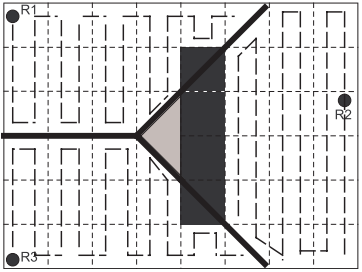
\includegraphics[scale=0.4]{figs/Voronoi_Euclid_BCD}
		\caption{Fig1}
		\label{fig:Voronoi - EuclidBCD}
	\end{subfigure}
	\hfill
	\begin{subfigure}[b]{0.45\textwidth}
		\centering
		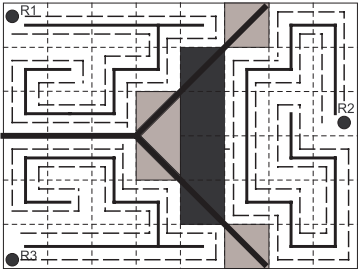
\includegraphics[scale=0.4]{figs/Voronoi_Euclid_STC}
		\caption{Fig2}
		\label{fig:Voronoi - EuclidSTC}
	\end{subfigure}
\caption{}
\end{figure}

\subsection{Negotiation Protocol}
A negotiation or bargaining protocol refers to a process involving task partitioning. In the context of area division for CPP, the task represents the area to be divided\cite{Rossi2009}. The authors of \cite{Rossi2009} present a negotiation model based on Rubinstein's alternate-offers protocol, for the purpose of area division. The focus of their implementation was to develop a distributed algorithm capable of considering robot capabilities. This means that the robots wouldn't have to be homogeneous and can have different flight-time capabilities, maneuverability, on-board equipment and so forth \cite{Barrientos2011}. 

They implemented their algorithm and found that it can achieve near optimum results. It tries to maximise the size of each robot's subdivision of the area (based on its capabilities), while also minimising sub-area overlap. The algorithm also works to avoid static obstacles or no fly zones that are present in the area. Moreover, they proved that it could be applied in a situation where re-planning may be necessary.
% Re-planning is necessary in a scenario when carrying out the plan changes the environment, thereby requireing replanning wiht the new environment scenario
% TODO: Future work - as new information about target becomes available - replan

A more complete implementation of the algorithm including an individual area search technique was also developed and tested \cite{Barrientos2011}. In this implementation they use a wavefront planner for the individual area coverage path generation. This requires discretisation of the area into cells. In their case, they used rectangles whose size was determined by on-board camera field of view (FOV). In order for the polygons generated by the negotiation protocol to work effectively, they use a method called Bresenham's line algorithm to approximate the lines that divide the areas in discrete space, so that they pass through the centroids of cells.

The area division achieved sometimes produces non-convex shapes, which the wavefront planner can handle effectively. Their implementation also minimizes energy consumption by minimizing the number of turns and not allowing backtracking. They also have the ability to specify the initial take-off positions of the robots. Distance from the specified take-off point to the starting point for sub-area coverage are considered in the sub-task negotiations. The authors also mention being able to specify robot landing positions preemptively.

One visible drawback in their implementation is that they coverage appears incomplete. The boundaries between areas pass through waypoints (cell centroids), that effectively get excluded from the coverage algorithm and are not covered. Using an exact method to search the individual areas could produce better results. Changing the boundaries to lie on the edges of cells rather than passing through their centroids could also make a difference.

\subsection{MSTC and MFC} 
Multi-robot spanning-tree coverage (MSTC) is a variant of single robot spanning tree coverage (STC) as presented in section \ref{sec:lit SR CPP - STC}. The authors of \cite{Hazon2005} designed the first variants of MSTC. The two variations they suggest are one that allows for backtracking and one that does not. Both variations still utilize a single spanning tree, but simply circumnavigate the tree with multiple robots instead of a single one.

They place a lot of emphasis on robustness and efficiency, in addition to completeness. They demonstrate an algorithm that segments the path around a spanning tree to evenly distribute it among robots. This distribution of robots is however, unrealistic. Their method becomes incredibly inefficient when robots are clustered closely together. This is because a robot simply navigates the path until it reaches the initial position of the next robot on the path. Figure \ref{fig:MSTC} shows the paths that are generated when the robots are evenly distributed along the path that circumnavigates the tree. Blue dots represent the robot initial positions and the spanning tree is shown in red. The second method they suggest remedies this somewhat. It allows for backtracking and improves the efficiency; which implies decreasing the time to completion.

The ideal situation is that all the robots have near equal path lengths, provided they are homogeneous robots. This is not guaranteed with this algorithm when the robots have random starting positions, but allowing for backtracking can improve the results and allow the coverage to be completed in a shorter amount of time. 

\begin{figure}
	\centering
	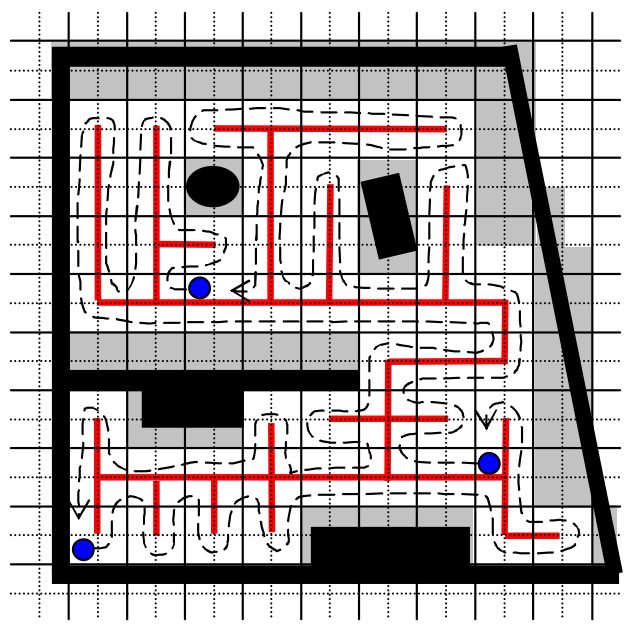
\includegraphics[scale=0.4]{figs/MSTC-Graphic}
	\caption{MSTC algorithm showing the paths for three robots on an environment grid. \cite{Hazon2005}}
	\label{fig:MSTC}
\end{figure}

\subsection{DARP}

%%%%%%%%%%%%%%%%%%%%%%%%%%%%%%%%%%%%%%%%%%%%%%%%%%%%%%%%%%%%%%%%%%%%%%%
\section{Non-Distributed Offline MCPP}
\subsection{Sampling-Based}
% Check Lavalle
\subsection{Artificial-Intelligence-Based}

%%%%%%%%%%%%%%%%%%%%%%%%%%%%%%%%%%%%%%%%%%%%%%%%%%%%%%%%%%%%%%%%%%%%%%%
\section{Online MCPP}

%%%%%%%%%%%%%%%%%%%%%%%%%%%%%%%%%%%%%%%%%%%%%%%%%%%%%%%%%%%%%%%%%%%%%%%

\section{UAVs and Search and Rescue}
%DroneSAR
%Rotary Wing vs Fixed-Wing UAVs}


